% =============================================================================
% AXI wiring of AccelShell -- standalone TikZ figure
% Compile:  pdflatex accel_shell_wiring.tex
% Include in a report:  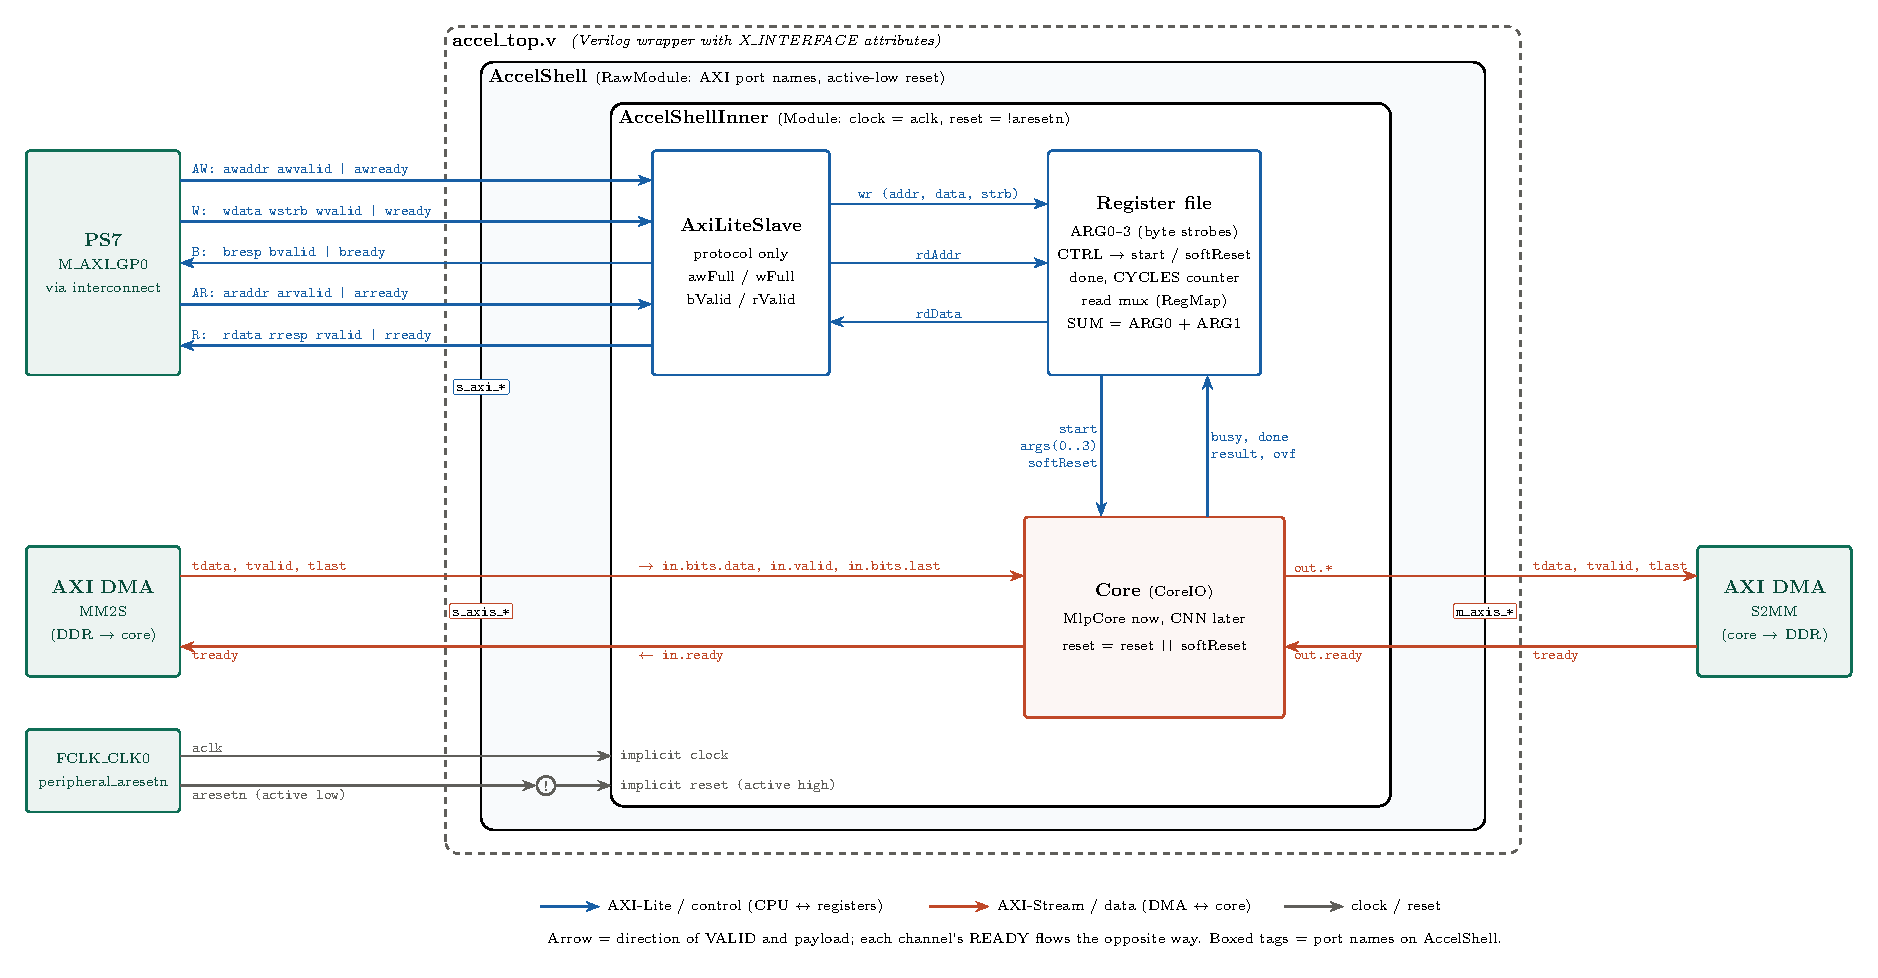
\includegraphics[width=\textwidth]{accel_shell_wiring.pdf}
% =============================================================================
\documentclass[tikz,border=8pt]{standalone}
\usetikzlibrary{arrows.meta,positioning,calc,backgrounds}

\definecolor{ctrl}{HTML}{185FA5}   % AXI-Lite / control path
\definecolor{data}{HTML}{C04828}   % AXI-Stream / data path
\definecolor{clk}{HTML}{5F5E5A}    % clock and reset
\definecolor{ext}{HTML}{0F6E56}    % Xilinx IP outside our design

\tikzset{
  >={Stealth[length=2.2mm]},
  blk/.style={draw, thick, rounded corners=2pt, align=center, inner sep=4pt, font=\small},
  extblk/.style={blk, draw=ext, fill=ext!8, text=ext!70!black, minimum width=2.6cm},
  mod/.style={blk, fill=white},
  sig/.style={font=\scriptsize\ttfamily, inner sep=1.5pt},
  port/.style={sig, fill=white, draw, rounded corners=1pt},
  c/.style={->, thick, draw=ctrl},
  d/.style={->, thick, draw=data},
  k/.style={->, thick, draw=clk},
  ttl/.style={font=\small\bfseries, anchor=north west, inner sep=3pt},
  sub/.style={font=\scriptsize\itshape, anchor=north west, inner sep=3pt},
}

\begin{document}
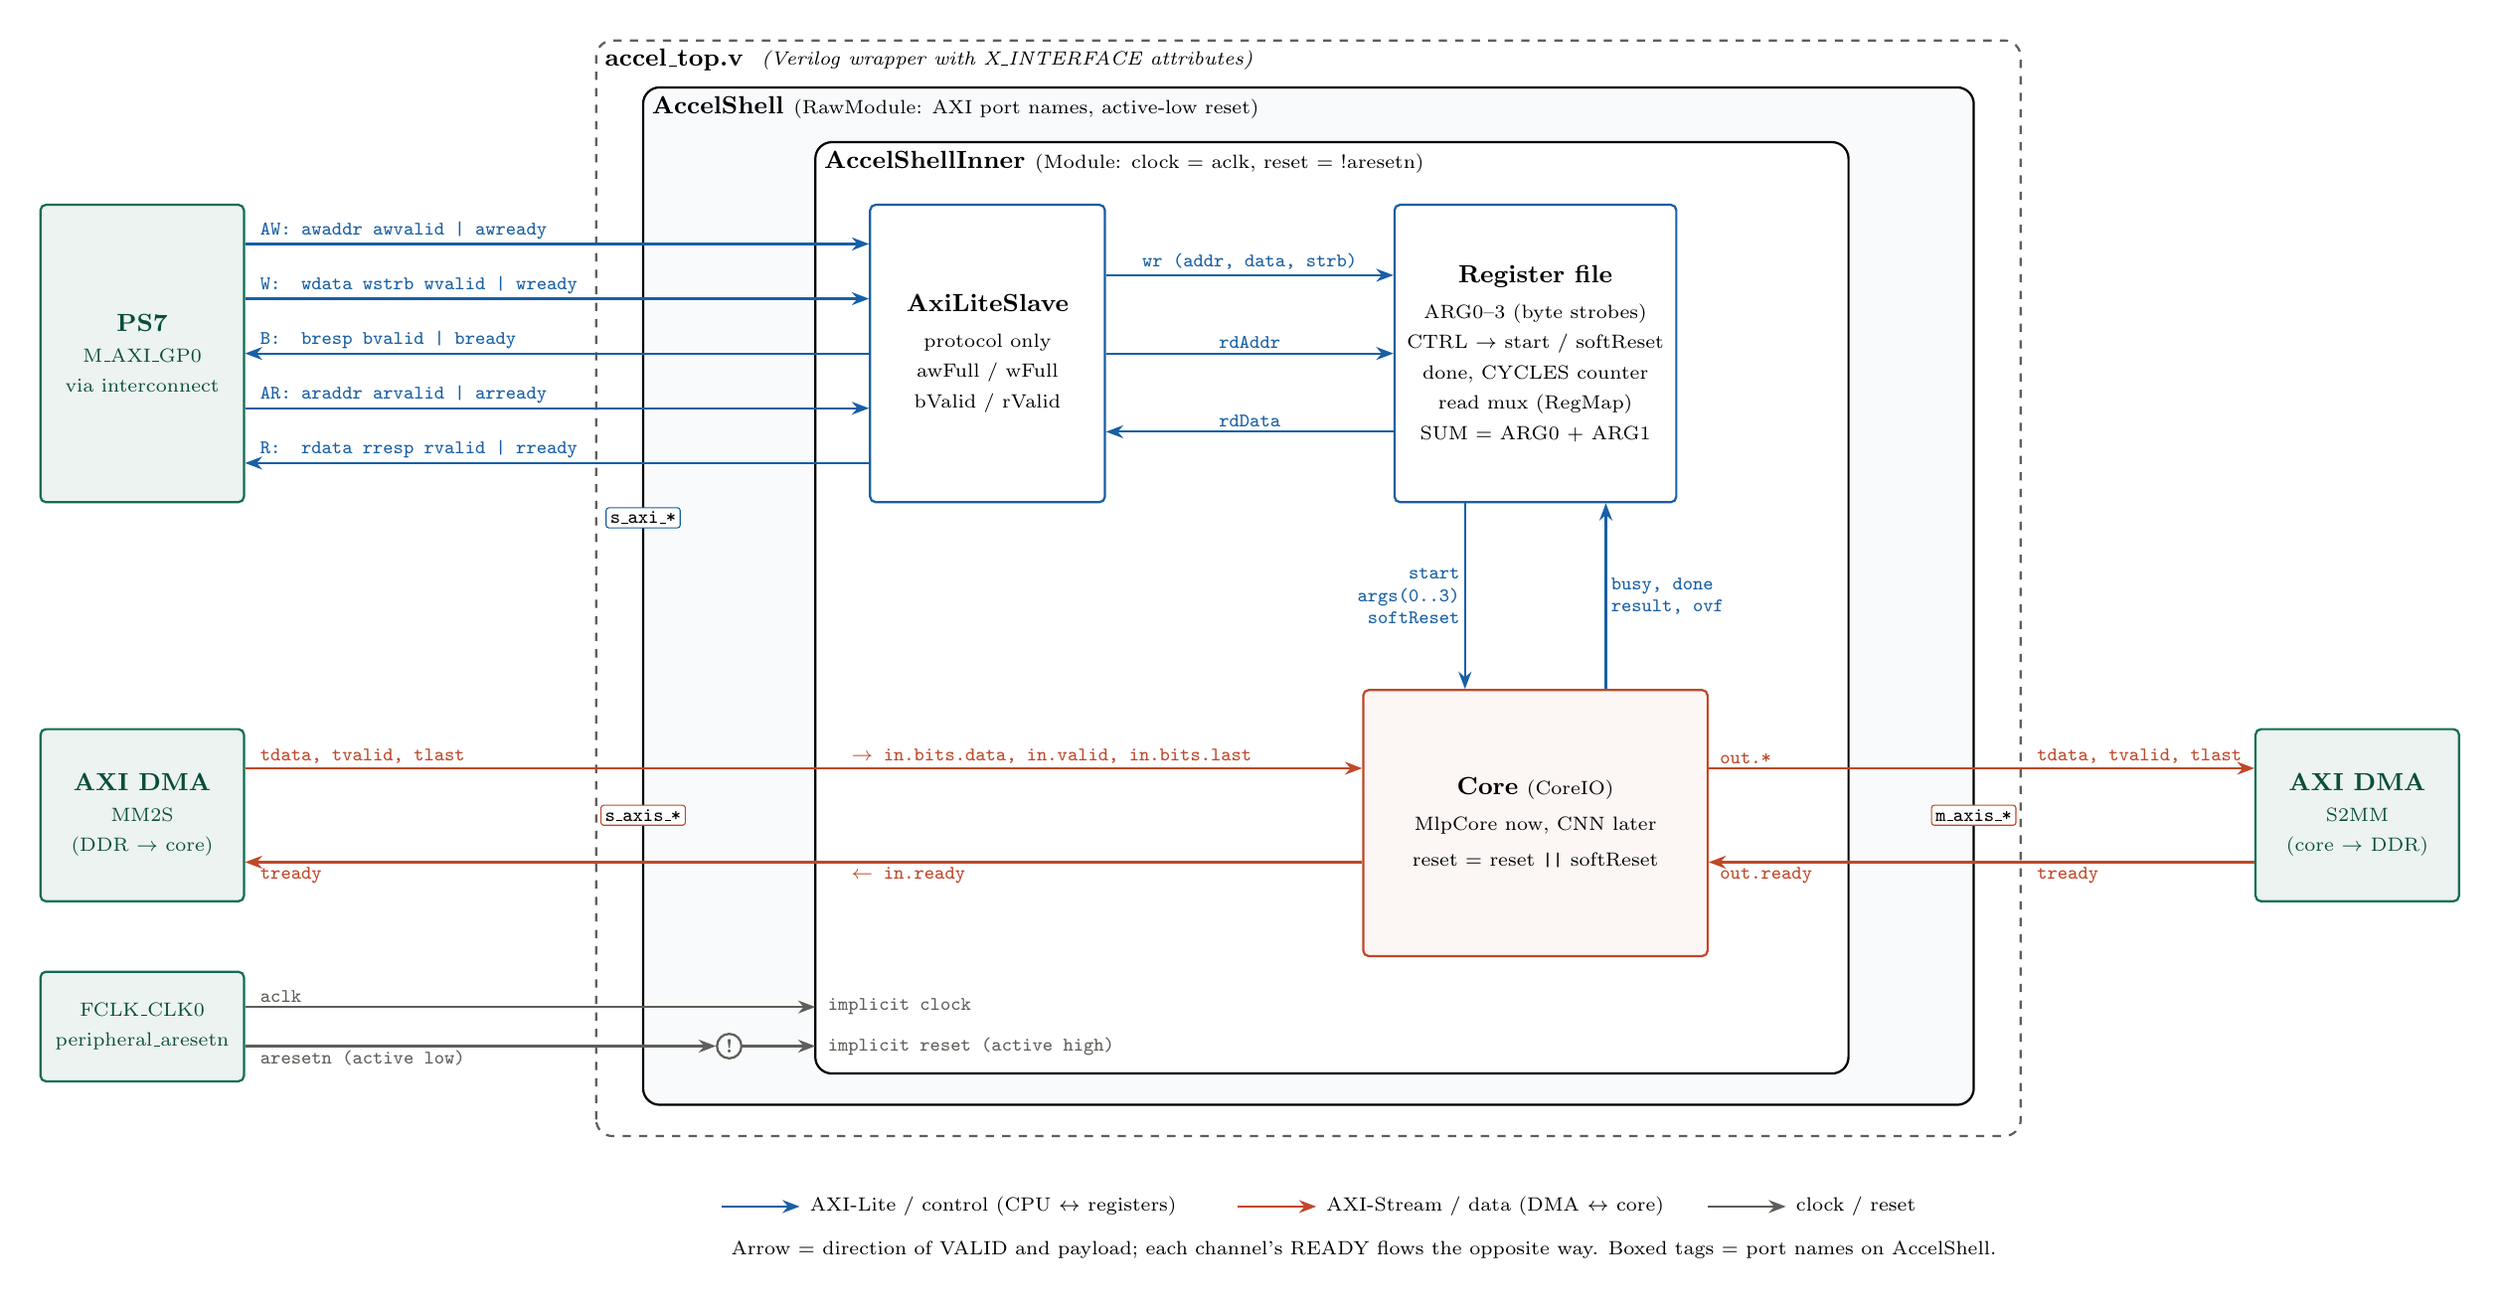
\begin{tikzpicture}[show background rectangle, background rectangle/.style={fill=white}]

% ---------------------------------------------------------------- containers
\draw[thick, dashed, rounded corners=6pt, draw=clk] (2.4,-3.4) rectangle (20.6,10.6);
\node[ttl] at (2.4,10.6) {accel\_top.v};
\node[sub] at (4.4,10.58) {(Verilog wrapper with X\_INTERFACE attributes)};

\draw[thick, rounded corners=6pt, fill=ctrl!3] (3.0,-3.0) rectangle (20.0,10.0);
\node[ttl] at (3.0,10.0) {AccelShell \normalfont\scriptsize(RawModule: AXI port names, active-low reset)};

\draw[thick, rounded corners=6pt, fill=white] (5.2,-2.6) rectangle (18.4,9.3);
\node[ttl] at (5.2,9.3) {AccelShellInner \normalfont\scriptsize(Module: clock = aclk, reset = !aresetn)};

% ---------------------------------------------------------------- inner modules
\node[mod, draw=ctrl, minimum width=3.0cm, minimum height=3.8cm] (slv) at (7.4,6.6)
  {\textbf{AxiLiteSlave}\\[2pt]\scriptsize protocol only\\\scriptsize awFull / wFull\\\scriptsize bValid / rValid};

\node[mod, draw=ctrl, minimum width=3.6cm, minimum height=3.8cm] (reg) at (14.4,6.6)
  {\textbf{Register file}\\[2pt]\scriptsize ARG0--3 (byte strobes)\\\scriptsize CTRL $\rightarrow$ start / softReset\\\scriptsize done, CYCLES counter\\\scriptsize read mux (RegMap)\\\scriptsize SUM = ARG0 + ARG1};

\node[mod, draw=data, fill=data!5, minimum width=4.4cm, minimum height=3.4cm] (core) at (14.4,0.6)
  {\textbf{Core} \scriptsize(CoreIO)\\[2pt]\scriptsize MlpCore now, CNN later\\[2pt]\scriptsize reset = reset \texttt{||} softReset};

% ---------------------------------------------------------------- external blocks
\node[extblk, minimum height=3.8cm] (gp0)  at (-3.4,6.6)  {\textbf{PS7}\\\scriptsize M\_AXI\_GP0\\\scriptsize via interconnect};
\node[extblk, minimum height=2.2cm] (mm2s) at (-3.4,0.7)  {\textbf{AXI DMA}\\\scriptsize MM2S\\\scriptsize (DDR $\rightarrow$ core)};
\node[extblk, minimum height=1.4cm] (rst)  at (-3.4,-2.0) {\scriptsize FCLK\_CLK0\\\scriptsize peripheral\_aresetn};
\node[extblk, minimum height=2.2cm] (s2mm) at (24.9,0.7)  {\textbf{AXI DMA}\\\scriptsize S2MM\\\scriptsize (core $\rightarrow$ DDR)};

% ---------------------------------------------------------------- AXI-Lite: 5 channels
% arrow = direction of VALID + payload; the READY of each channel goes the other way
\foreach \y/\lbl/\dir in {8.0/AW: awaddr awvalid | awready/1,
                          7.3/W:\ \ wdata wstrb wvalid | wready/1,
                          6.6/B:\ \ bresp bvalid | bready/0,
                          5.9/AR: araddr arvalid | arready/1,
                          5.2/R:\ \ rdata rresp rvalid | rready/0} {
  \ifnum\dir=1
    \draw[c] (gp0.east |- 0,\y) -- (slv.west |- 0,\y);
  \else
    \draw[c] (slv.west |- 0,\y) -- (gp0.east |- 0,\y);
  \fi
  \node[sig, text=ctrl, anchor=south west] at (-1.95,\y) {\lbl};
}
\node[port, draw=ctrl] at (3.0,4.5) {s\_axi\_*};

% slave <-> register file
\draw[c] (slv.east |- 0,7.6) -- (reg.west |- 0,7.6) node[sig, midway, above, text=ctrl] {wr (addr, data, strb)};
\draw[c] (slv.east |- 0,6.6) -- (reg.west |- 0,6.6) node[sig, midway, above, text=ctrl] {rdAddr};
\draw[c] (reg.west |- 0,5.6) -- (slv.east |- 0,5.6) node[sig, midway, above, text=ctrl] {rdData};

% register file <-> core
\draw[c] ([xshift=-0.9cm]reg.south) -- ([xshift=-0.9cm]core.north)
  node[sig, midway, left, text=ctrl, align=right] {start\\args(0..3)\\softReset};
\draw[c] ([xshift=0.9cm]core.north) -- ([xshift=0.9cm]reg.south)
  node[sig, midway, right, text=ctrl, align=left] {busy, done\\result, ovf};

% ---------------------------------------------------------------- AXI-Stream in (s_axis)
\draw[d] (mm2s.east |- 0,1.3) -- (core.west |- 0,1.3);
\draw[d] (core.west |- 0,0.1) -- (mm2s.east |- 0,0.1);
\node[sig, text=data, anchor=south west] at (-1.95,1.3) {tdata, tvalid, tlast};
\node[sig, text=data, anchor=north west] at (-1.95,0.1) {tready};
\node[sig, text=data, anchor=south west] at (5.6,1.3) {$\rightarrow$ in.bits.data, in.valid, in.bits.last};
\node[sig, text=data, anchor=north west] at (5.6,0.1) {$\leftarrow$ in.ready};
\node[port, draw=data] at (3.0,0.7) {s\_axis\_*};

% ---------------------------------------------------------------- AXI-Stream out (m_axis)
\draw[d] (core.east |- 0,1.3) -- (s2mm.west |- 0,1.3);
\draw[d] (s2mm.west |- 0,0.1) -- (core.east |- 0,0.1);
\node[sig, text=data, anchor=south west] at (16.7,1.3) {out.*};
\node[sig, text=data, anchor=north west] at (16.7,0.1) {out.ready};
\node[sig, text=data, anchor=south west] at (20.75,1.3) {tdata, tvalid, tlast};
\node[sig, text=data, anchor=north west] at (20.75,0.1) {tready};
\node[port, draw=data] at (20.0,0.7) {m\_axis\_*};

% ---------------------------------------------------------------- clock / reset
\node[draw=clk, thick, circle, inner sep=1.2pt, font=\scriptsize\bfseries, text=clk] (inv) at (4.1,-2.25) {!};
\draw[k] (rst.east |- 0,-1.75) -- (5.2,-1.75);
\draw[k] (rst.east |- 0,-2.25) -- (inv.west);
\draw[k] (inv.east) -- (5.2,-2.25);
\node[sig, text=clk, anchor=south west] at (-1.95,-1.75) {aclk};
\node[sig, text=clk, anchor=north west] at (-1.95,-2.25) {aresetn (active low)};
\node[sig, text=clk, anchor=west] at (5.3,-1.75) {implicit clock};
\node[sig, text=clk, anchor=west] at (5.3,-2.25) {implicit reset (active high)};

% ---------------------------------------------------------------- legend
\begin{scope}[shift={(4.0,-4.3)}]
  \draw[c] (0,0) -- (1,0) node[right, font=\scriptsize, text=black] {AXI-Lite / control (CPU $\leftrightarrow$ registers)};
  \draw[d] (6.6,0) -- (7.6,0) node[right, font=\scriptsize, text=black] {AXI-Stream / data (DMA $\leftrightarrow$ core)};
  \draw[k] (12.6,0) -- (13.6,0) node[right, font=\scriptsize, text=black] {clock / reset};
  \node[font=\scriptsize, anchor=west] at (0,-0.55)
    {Arrow = direction of VALID and payload; each channel's READY flows the opposite way. Boxed tags = port names on AccelShell.};
\end{scope}

\end{tikzpicture}
\end{document}
